% -------------------------------- PREAMBLE --------------------------------
\documentclass[a4paper]{report}

\usepackage[utf8]{inputenc}
\usepackage{graphicx}
\usepackage{tikz}
\usepackage{booktabs}
\usepackage[format=hang,font=small,labelfont=bf]{caption}
\usepackage[protrusion=true,expansion=true]{microtype}
\usepackage{amsmath}
\usepackage{amssymb}
\usepackage{amsthm}
\usepackage{upgreek}
\usepackage{nbaseprt}
\usepackage{appendix}
\usepackage{color}
\usepackage{url}
\usepackage{hyperref}
\usepackage{underscore}
\usepackage[numbers]{natbib}
\usepackage{enumitem}
\usepackage{algorithm}
\usepackage{algorithmicx}
\usepackage{algpseudocode}

\newcommand{\reporttitle}{Metric Based Data Analysis Techniques}
\newcommand{\reportauthor}{George Kettleborough}

% --- hyperref stuff ---
\definecolor{darkblue}{rgb}{0,0,0.4}
\hypersetup{
  pdftex,
  bookmarks=true,
  bookmarksopen=true,
  colorlinks=true,
  citecolor=black,
  filecolor=black,
  linkcolor=black,
  urlcolor=darkblue,
  pdfauthor={\reportauthor},
  pdftitle={\reporttitle},
  pdfsubject={}
}
\providecommand{\doi}[1]{\href{http://dx.doi.org/#1}{doi: #1}}

% --- TikZ stuff ---

\usetikzlibrary{calc,trees,positioning,arrows,chains,shapes.geometric,%
  decorations.pathreplacing,decorations.pathmorphing,shapes,%
  matrix,shapes.symbols}

% --- End TikZ stuff ---


% the figures location
\graphicspath{./figures/}

% make equations and figures numbered (sec.eq)
% \numberwithin{equation}{section}
% \numberwithin{figure}{section}

% new operators for maths
\DeclareMathOperator{\op}{op}
\DeclareMathOperator{\remainder}{remainder}
\DeclareMathOperator{\lc}{lc}
\DeclareMathOperator{\pquo}{pquo}
\DeclareMathOperator{\prem}{prem}
\DeclareMathOperator{\pp}{pp}
\DeclareMathOperator{\cont}{cont}
\DeclareMathOperator{\resultant}{resultant}
\DeclareMathOperator{\numerator}{numerator}
\DeclareMathOperator{\denominator}{denominator}
\DeclareMathOperator{\ADCO}{ADCO}
\DeclareMathOperator{\dens}{dens}
\DeclareMathOperator{\symdif}{\bigtriangleup}
\DeclareMathOperator*{\argmin}{arg\,min}

\newcommand{\dset}{\mathcal{D}}
\newcommand{\clus}{\mathcal{C}}
\newcommand{\NP}{\text{NP}}

% theorems
\newtheorem{thm}{Theorem}
\newtheorem{lem}{Lemma}
\newtheorem{cor}{Corollary}
\newtheorem{dfn}{Definition}

% problem template
\newenvironment{problem}[1]{\par\addvspace{\topsep}\noindent\textsc{#1}\\}
{\par\addvspace{\topsep}}
\newcommand{\instance}[1]{\textsc{Instance:} #1\\}
\newcommand{\question}[1]{\textsc{Question:} #1}

\title{\reporttitle}
\author{\reportauthor}

% ------------------------------ END PREAMBLE ------------------------------

\begin{document}

\maketitle

\tableofcontents

\chapter{Introduction}
\label{cha:introduction}

\chapter{Background}
\label{cha:background}

\section{Summary}
\label{sec:summary-backgd}


\section{Datasets and metric spaces}
\label{sec:datas-metr-spac}

Let $M$ be a set and $d \colon M \times M \to \mathcal{R}$ a function where,
for all $x,y \in M$, the following conditions hold
\begin{enumerate}
\item $d(x,y) \geq 0$,
\item $d(x,y) = d(y,x)$,
\item
  \begin{enumerate}
  \item $d(x,x) = 0$.
  \end{enumerate}
\end{enumerate}
Such a function is called a distance and can be used to measure the similarity
between elements of $M$: closer elements are more similar and distant elements
less similar.  If we add two more conditions, namely, for all $x,y,z \in M$,
\begin{enumerate}[start=3]
\item
  \begin{enumerate}[start=2]
  \item $d(x,y) = 0$ only if $x=y$,
  \end{enumerate}

\item $d(x,y) + d(y,x) \geq d(x,z)$,
\end{enumerate}
then $d$ is also a \textit{metric} and the ordered pair $(M,d)$ is called a
\textit{metric space}.

A metric is the most intuitive type of dissimilarity measure for human use.
In a metric space, for example, if we know that some object $a$ is distant
from some object $b$, and we know that another object $c$ is close to $b$,
then it is natural for us to make the deduction that $c$ is also distant from
$a$.  This deduction would be incorrect in a general distance space.

A dataset is simply a collection of data.  These data usually arise as the
result of an experiment, for example the classic iris dataset arose from
measuring parts of certain flowers.  One of the first things one might wish to
do with such a dataset is compare its elements.

One way to do this is to invent a metric for the dataset.  If the elements are
of a common type, such as real valued vectors, then an existing metric can be
used, for example the well known Euclidean metric.

It is tempting to think of the dataset and some metric as a metric space, but
this is not strictly correct.  The reason is that, contrary to the name, a
dataset if not generally a set, but a multiset.  In other words, identical
elements can appear more than once.  We therefore define a dataset to be a
multiset $(\dset, \mu_{\dset})$ where $\dset$ is called the underlying set and
$\mu_{\dset} \colon \dset \to \mathbb{Z}^+$ is called the membership function
and maps each element of $\dset$ to its multiplicity.  If $d$ is a metric
defined for all elements in $\dset$, then $(\dset, d)$ is a metric space.

For the purposes of discussion we will only explicitly treat a dataset as a
multiset when it is necessary.  Normally we will just work on $\dset$ directly
and assume that $\mu_{\dset}(x) = 1$ for all $x \in \dset$.

\section{Partitions}
\label{sec:partitions}

In this section we look at the properties of partitions of datasets, how we
can compare partitions and how we can find partitions.

\subsection{The space of partitions}
\label{sec:space-partitions}

A partition of a (multiset) dataset, $(\dset,\mu_{\dset})$, is a set of $k$
multisets, $\{(C_1,\mu_1),(C_2,\mu_2),\dotsc,(C_k,\mu_k)\}$ where $C_1 \cup
C_2 \cup \dotsb \cup C_k = \dset$, for all $i = 1,\dotsc,k, \sum_{x \in \dset}
\mu_i(x) > 0$ and, for all $x \in \dset$, $\sum_{i=1}^{k} \mu_i(x) =
\mu_{\dset}(x)$.  In other words, it is a set of nonempty, nonoverlapping
subsets.  These subsets are called clusters.

\begin{figure}
  \centering
  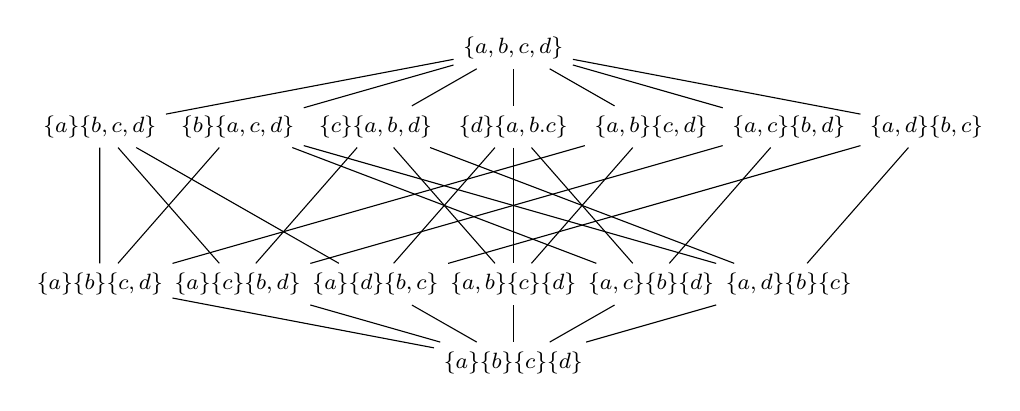
\begin{tikzpicture}[
    xscale=1.75, font=\footnotesize]

    % vertices
    
    \node (0) at (0,0) {$\{a,b,c,d\}$};

    \node (10) at (-3,-1) {$\{a\}\{b,c,d\}$};
    \node (11) at (-2,-1) {$\{b\}\{a,c,d\}$};
    \node (12) at (-1,-1) {$\{c\}\{a,b,d\}$};
    \node (13) at (0,-1) {$\{d\}\{a,b.c\}$};
    \node (14) at (1,-1) {$\{a,b\}\{c,d\}$};
    \node (15) at (2,-1) {$\{a,c\}\{b,d\}$};
    \node (16) at (3,-1) {$\{a,d\}\{b,c\}$};

    \node (20) at (-3,-3) {$\{a\}\{b\}\{c,d\}$};
    \node (21) at (-2,-3) {$\{a\}\{c\}\{b,d\}$};
    \node (22) at (-1,-3) {$\{a\}\{d\}\{b,c\}$};
    \node (23) at (0,-3) {$\{a,b\}\{c\}\{d\}$};
    \node (24) at (1,-3) {$\{a,c\}\{b\}\{d\}$};
    \node (25) at (2,-3) {$\{a,d\}\{b\}\{c\}$};

    \node (3) at (0,-4) {$\{a\}\{b\}\{c\}\{d\}$};

    % edges

    \draw (0) to (10);
    \draw (0) to (11);
    \draw (0) to (12);
    \draw (0) to (13);
    \draw (0) to (14);
    \draw (0) to (15);
    \draw (0) to (16);

    \draw (10) to (20);
    \draw (10) to (21);
    \draw (10) to (22);
    \draw (11) to (20);
    \draw (11) to (24);
    \draw (11) to (25);
    \draw (12) to (21);
    \draw (12) to (23);
    \draw (12) to (25);
    \draw (13) to (22);
    \draw (13) to (23);
    \draw (13) to (24);
    \draw (14) to (20);
    \draw (14) to (23);
    \draw (15) to (21);
    \draw (15) to (24);
    \draw (16) to (22);
    \draw (16) to (25);

    \draw (20) to (3);
    \draw (21) to (3);
    \draw (22) to (3);
    \draw (23) to (3);
    \draw (24) to (3);
    \draw (25) to (3);
  \end{tikzpicture}
  \caption{The lattice of partitions of dataset $\{a,b,c,d\}$ \citep{meila-2005}.}
  \label{fig:lattice}
\end{figure}

Let $\mathcal{P}_{\dset}$ be the set of all partitions of $\dset$.  The
natural way to represent the set $\mathcal{P}_{\dset}$ is as a graph called
the lattice of partitions.  Such a graph is shown in figure~\ref{fig:lattice}.
The top of the graph contains a single node containing $\hat{1} = \{\dset\}$
which is the partition with one cluster and the bottom is a single node
containing $\hat{0} = \{\{D_1\},\{D_2\},\dotsc,\{D_n\}\}$ the partition
containing $n$ clusters.

A partition, $\clus'$, which is obtained by splitting one or more clusters in
$\clus$ is said to be a refinement of $\clus$.  Every edge in the lattice
represents a refinement, with the coarser partition at the top.

As can be seen from figure~\ref{fig:lattice}, the number of possible
partitions for a 4 element dataset is already quite large; for a 20 element
dataset the number is more than 51 trillion.  In general the number of
possible partitions of an $n$ element dataset is equivalent to the $n$th Bell
number, $B_n$~\citep{bell1934exponential}.  The sequence of Bell numbers
begins with $B_0 = 1$ and its growth is then superexponential in $n$.  The
rest of sequence can be generated in a few ways including by a recursive
formula:
\begin{equation*}
  B_n = \sum_{k=0}^{n-1} B_k {n-1 \choose k},
\end{equation*}
or using Dobinski's formula:
\begin{equation*}
  B_n = \frac{1}{e} \sum_{k=0}^{\inf} \frac{k^n}{k!}.
\end{equation*}

\subsection{Comparing partitions}
\label{sec:comparing-partitions}

Since the space of possible partitions for any given dataset is very large, it
becomes useful to speak of similarity between different partitions.  It is
highly likely that different clustering algorithms will produce different
partitions given the same dataset, and some algorithms are non-deterministic,
for example $k$-means is often ``seeded'' with random clusters.  Such a
(dis)similarity measure could therefore be used to compare algorithms, or
assess the ability of a non-deterministic algorithm to consistently find good
solutions for hard problems.

It is quite easy to devise dissimilarity measures for partitions, but those
that are generally found most useful are distances, meaning they satisfy
conditions 1--3 of the metric definition.  If a dissimilarity measure further
satisfies condition~4 then it is also a metric.  A metric is the most
intuitive type of measure for human use.  In a metric space, for example, if
we know that some object $a$ is distant from some object $b$, and we know that
another object $c$ is close to $b$, then it is natural for us to make the
deduction that $c$ is also distant from $a$.  This deduction would be
incorrect in a general distance space.

We would argue that metrics are therefore the most desirable type of
dissimilarity measure.  Many metrics have been devised, and many more measures
that are not metrics or not even distances.  Existing measures fall into four
main categories which will each be discussed in the following subsections.
Briefly, these are:
\begin{description}
\item[Pair counting] which counts pairs of data points to measure the
  ``agreement'' and ``disagreement'' between two clusterings,
\item[Set matching] which matches clusters in one clustering to clusters in
  the other and measures the difference between these matched pairs,
\item[Information theoretic measures] which use information theory to
  describe the mutual information between two clusterings,
\item[Density profile based measures] which takes into account the attributes
  of the data set when determining similarity between clusterings.
\end{description}

As usual, let $\mathcal{D} = \{D_1,D_2,\dotsc,D_n\}$ be our data set and $P_1
= \{C_{11},C_{12},\dotsc,C_{1k}\}$ and $P_2 =
\{C_{21},C_{22},\dotsc,C_{2k'}\}$ be two partitions of $\mathcal{D}$.  The
contingency matrix of $P_1$ and $P_2$ is a $k \times k'$ matrix where the
$ij$-th element is $n_{ij} = |C_{1i} \cap C_{2j}|$.

\subsubsection{Pair counting}
\label{sec:pair-counting}

There are $\binom{n}{2}$ distinct pairs of objects in $\mathcal{D}$, and these
can be divided into four types:
\begin{description}
\item[$N_{11}$]: objects which are in the same cluster in $P_1$ and in the
  same cluster in $P_2$,
\item[$N_{00}$]: objects which are in different clusters in $P_1$ and in
  different clusters in $P_2$,
\item[$N_{10}$]: objects which are in the same cluster in $P_1$ but in
  different clusters in $P_2$,
\item[$N_{01}$]: objects which are in different clusters in $P_1$ but in the
  same cluster in $P_2$.
\end{description}

$N_{11}$ and $N_{00}$ are considered to be ``agreements'' and $N_{10}$ and
$N_{01}$ are ``disagreements''.  Clearly $N_{11} + N_{00} + N_{10} + N_{01} =
\binom{n}{2}$ is always satisfied.  The four counts can be obtained from the
confusion matrix \citep{fowlkes-mallows-1983}.

There are a number of different criteria that have been used in the literature
that are based on these counts.  The simplest of these are
$\mathcal{R}(P_1,P_2) = (N_{11}+N_{00})/\binom{n}{2}$ used by
\citet{rand-1971}; $(N_{10}+N_{01})/\binom{n}{2}$ used by Johnson, Mirkin,
Arabie and Boorman; and $(N_{11}+N_{00}-N_{10}-N_{01})/\binom{n}{2}$ used by
Hubert \citep{hubert-arabie-1985}.  The first of these, known as the Rand
index, is widely used and often cited in the literature.

\citet{fowlkes-mallows-1983} present a measure which they call $B_k$ for
comparing two hierarchical clusterings.  \citet{wallace-1983} later showed
that this measure could be stated in terms of two asymmetric measures
\begin{equation*}
  \mathcal{W}_{I}(P_1,P_2) = \frac{N_{11}}{\sum_{i=1}^{k}
    |C_{1i}|(|C_{1i}|-1)/2}
\end{equation*}
and
\begin{equation*}
  \mathcal{W}_{II}(P_1,P_2) = \frac{N_{11}}{\sum_{j=1}^{k'}
    |C_{2j}|(|C_{2j}|-1)/2},
\end{equation*}
which represent the probabilities that a pair of points which are in the same
cluster in $P_1$ and $P_2$ respectively, are also in the same cluster in the
other partition.  It was shown that Fowlkes and Mallows's original symmetric
measure is then simply the geometric mean of these two asymmetric measures
\citep{wallace-1983}
\begin{equation*}
  \mathcal{F}(P_1,P_2) = \sqrt{\mathcal{W}_{I}(P_1,P_2)\mathcal{W}_{II}(P_1,P_2)}.
\end{equation*}

The Jaccard coefficient \citep{ben-hur-2001} is an improved version of the
Rand index which is also well known and widely used
\begin{equation*}
  \mathcal{J}(P_1,P_2) = \frac{N_{11}}{N_{01}+N_{10}+N_{11}}.
\end{equation*}

So far, none of the measures listed are claimed to be metrics.  The Rand index
is clearly not a metric as it takes the value of $1$ for identical
clusterings.  In fact, the value of $N_{11}$ can always take a nonzero value
for identical clusterings.  Therefore both $\mathcal{F}$ and $\mathcal{J}$ are
not metrics as they are based on normalising the value of $N_{11}$.

One measure based on pair counting which is a metric is the Mirkin metric
\citep{mirkin-1996}
\begin{equation*}
  \mathcal{M}(P_1,P_2) = \sum_{i=1}^{k} |C_{1i}|^2 + \sum_{j=1}^{k'} |C_{2j}|^2
  - 2 \sum_{i=1}^{k} \sum_{j=1}^{k'} n_{ij}^2.
\end{equation*}
This can also be written as
\begin{equation*}
  \mathcal{M}(P_1,P_2) = 2(N_{01} + N_{10}) = n(n-1)(1-\mathcal{R}(P_1,P_2))
\end{equation*}
and is therefore an adjusted form of the Rand index \citep{meila-2007}.  In
fact, it turns out that the Rand index has been independently rediscovered in
different forms by many different authors \citep{hubert-arabie-1985}.

\subsubsection{Set matching}
\label{sec:set-matching}

These measures are based on the cardinality of the intersect of ``matched''
clusters.  \citet{meila-2001} present a method which finds a matching using a
heuristic: the greatest value in the contingency table, $n_{ab}$, is taken as
the first match, then the greatest value not in either row $a$ or column $b$
is the second match, and so on.  The function $match(i)$ gives the index of
the cluster in $P_2$ which matches cluster $C_{1i}$ by this heuristic.  The
measure is then
\begin{equation*}
  \mathcal{H}(P_1,P_2) = \frac{1}{n} \sum_{j=match(i)} n_{ij}.
\end{equation*}
A second measure used by \citet{larsen-aone-1999} is
\begin{equation*}
  \mathcal{L}(P_1,P_2) = \frac{1}{k} \sum_{i=1}^{k} \max_{j}
  \frac{2n_{ij}}{|C_{1i}|+|C_{2j}|}.
\end{equation*}
Neither of these are metrics.

The following was introduced by \citet{van-dongen-2000} and is a metric
\begin{equation*}
  \mathcal{D}(P_1,P_2) = 2n - \sum_{i=1}^{k} \max_{j} n_{ij} - \sum_{j=1}^{k'}
  \max_{i} n_{ij}.
\end{equation*}

\citet{meila-2005} introduces another metric called classification error which
they define as
\begin{equation*}
  d_{CE}(P_1,P_2) = 1 - \frac{1}{n} \max_{\sigma} \sum_{i=1}^{K} n_{i\sigma(i)}
\end{equation*}
where $K = \min(k,k')$.  Calculation of this metric requires finding a maximum
matching which can be done in polynomial time.  This metric is bounded by
$[0,1]$ but it ignores $k-k'$ clusters whenever $k>k'$ and vice versa.  The
proof that it is a metric is not provided in the paper.

\citet{meila-2007} points out that all of these measures suffer from the
so-called ``problem of matching''.  Given a clustering $P_1$ we can obtain a
second clustering $P_2$ by moving a fraction $f$ of the objects from each
cluster $C_i$ to $C_{(i+1)\bmod k}$.  We then obtain a third clustering $P_3$
from $P_1$ by reassigning the same fraction $f$ of objects from each cluster
evenly among the other clusters.  It is claimed that $P_3$ is intuitively a
less disrupted version of $P_1$ than $P_2$ is, but $\mathcal{H}(P_1,P_2) =
\mathcal{H}(P_1,P_3) = \mathcal{L}(P_1,P_2) = \mathcal{L}(P_1,P_3) =
\mathcal{D}(P_1,P_2) = \mathcal{D}(P_1,P_3)$ whenever $f < \frac{1}{2}$.

A similar problem is pointed out in \citet{bae-2010}.  However, it appears
that utilising the underlying metric space of the data would alleviate this
problem, but this is not discussed in the literature.

\subsubsection{Information theoretic}
\label{sec:inform-theor}

Two measures which use information theory are Normalized Mutual Information
(NMI) \citep{fred-jain-2003} and Variation of Information (VI)
\citep{meila-2007}.  These measures essentially show how much information one
clustering contains about the other \citep{bae-2010}.

\citet{meila-2005} compares some of these methods by viewing all possible
partitions of a data set as a lattice.  Five axioms are introduced which are
satisfied by VI.  Other methods are shown to satisfy some of these axioms.
A distance measure is said to ``align'' with the lattice if the distances can
be expressed in terms of a sum of distances along the edges of the lattice.
VI is shown to align with the lattice while classification error is shown to
be not aligned.

The variation of information is based on both how much information is
contained in each clustering and how much information one clustering contains
about the other.  The entropy associated with a clustering $P_1$ is defined as
\begin{equation*}
  H(P_1) = - \sum_{i=1}^{k} P_1(i) \log P_1(i)
\end{equation*}
where
\begin{equation*}
  P_1(i) = \frac{|C_{1i}|}{k} \quad \text{for $i = 1, \dotsc, k$}
\end{equation*}
which is the probability that an object picked randomly from $\mathcal{D}$
belongs to cluster $C_{1i}$.  The entropy tells us the uncertainty about which
cluster an object in $\mathcal{D}$ belongs to.

The mutual information between two clusterings, $P_1$ and $P_2$, is defined as
\begin{equation*}
  I(P_1,P_2) = \sum_{i=1}^{k} \sum_{j=1}^{k'} P_{12}(i,j)
  \log \frac{P_{12}(i,j)}{P_{1}(i) P_{2}(j)}
\end{equation*}
where
\begin{equation*}
  P_{12}(i,j) = \frac{|C_{1i} \cap C_{2j}|}{n}
\end{equation*}
which is the probability that an object picked randomly from $\mathcal{D}$ is
in both $C_{1i}$ in $P_1$ and $C_{2j}$ in $P_2$.

Variation of information is then defined as
\begin{equation*}
  VI(P_1,P_2) = H(P_1) + H(P_2) - 2I(P_1,P_2).
\end{equation*}
This is a metric \citep{meila-2007}.  It is also $n$-invariant which means it
depends only on the relative sizes of the clusters, not on the number of
objects in $\mathcal{D}$.

The metric is bounded for all $n$ by
\begin{equation*}
  VI(P_1,P_2) \leq \log n.
\end{equation*}
Also, if the number of clusters in each partition is at most $k^{*}$, where
$k^{*} \leq \sqrt{n}$ then the following bound is attained
\begin{equation*}
  VI(P_1,P_2) \leq 2 \log k^{*}.
\end{equation*}

\subsubsection{Density based}
\label{sec:density-based}

So far none of the measures we have seen have taken into account the
attributes of the data set, or that the data set itself is a metric space.
The Attribute Distribution Clustering Orthogonality (ADCO) measure uses
density profiles based on the attributes of the data set to measure the
similarity between clusterings \citep{bae-2010}.  This solves a few problems
with other techniques including the ``problem of matching'' mentioned in
section~\ref{sec:set-matching}.

To compute the measure, first each attribute of the data set is split into the
same number of bins.  Then a density profile vector is created for each
clustering based on the number of objects in each bin belonging to each
cluster.  The measure then takes the dot-product of one vector and a
transformation of the other vector.  The transformation is performed by a
maximum assignment function which is computed using the Hungarian algorithm in
$O(K_{\min}^3)$ time, where $K_{\min} = \min(k,k')$ \citep{bae-2010}.

The $\ADCO$ function itself is a non-negative similarity measure which takes a
higher value when clusterings are more similar.  This can be converted into a
distance measure defined as
\begin{equation*}
  D_{\ADCO}(P_1,P_2) =
  \begin{cases}
    2 - \ADCO(P_1,P_2) & \qquad \text{if $P_1 \neq P_2$},\\
    0 & \qquad \text{otherwise}.
  \end{cases}
\end{equation*}
The first case is true whenever the density profile vectors of each clustering
are not equal.  $D_{\ADCO}$ is a metric \citep{bae-2010}.

\section{Partional clustering}
\label{sec:part-clust-algor}

We now turn to the problem of finding meaningful partitions of a dataset.
This problem is known as partitional clustering.

Applications for partitional clustering appear in nearly all natural sciences
and other fields such as computer science, engineering and market research.
The applications generally fall into two main categories: data reduction and
object classification.

Data reduction is often employed if a dataset is very large and one wishes to
capture only the essence of the data.  The essence will then be easier to
display or perform statistical analysis on, for example.  Object
classification is used in areas such as machine learning where one wishes to
give labels to newly observed instances based on some training data.

The following subsections first look at criteria which are used for judging
the suitability of a partition and then look at the complexity issues
associated with finding optimal clusterings according to one of these
criteria.  Finally we look at actual methods which are in use to perform
partitional clustering.

\subsection{Criteria}
\label{sec:criteria}

Judging the suitability of a particular partition is often a highly subjective
task but, nevertheless, many objective criteria have been devised for the
purpose of clustering.  In general, a partition is considered to be good if
the clusters are both homogeneous, meaning elements belonging to the same
cluster are similar, and well-separated, meaning elements belonging to
different clusters are dissimilar.  Given a criterion, the problem of
clustering then becomes attempting to find the partition which minimises or
maximises that criterion.

Let $\clus = \{C_1,C_2,\dotsc,C_k\}$ be a partition of dataset $\dset$ with a
dissimilarity measure $d$.  The following criteria measure the homogeneity of
a particular cluster, $C_i$.  The diameter is the maximum dissimilarity
between two members of the cluster:
\begin{equation*}
  \max_{x,y \in C_i} d(x,y).
\end{equation*}
The radius is the minimum of the maximum dissimilarities between each member
and another member of the cluster:
\begin{equation*}
  \min_{x \in C_i} \max_{y \in C_i} d(x,y).
\end{equation*}
The star is the minimum of the sums of dissimilarities between each member and
every other member of the cluster:
\begin{equation*}
  \min_{c \in C_i} \sum_{x \in C_i} d(c,x).
\end{equation*}
The clique is the sum of dissimilarities between each pair of members of the
cluster:
\begin{equation*}
  \sum_{x,y \in C_i} d(x,y).
\end{equation*}

The following criteria measure the separation of a cluster, $C_i$.  The split
is the minimum dissimilarity between a member of the cluster and an element
outside of the cluster:
\begin{equation*}
  \min_{x \in C_i, y \in \dset \setminus C_i} d(x,y).
\end{equation*}
The cut is the sum of dissimilarities between all members of the cluster and
all elements outside of the cluster:
\begin{equation*}
  \sum_{x \in C_i} \sum_{y \in \dset \setminus C_i} d(x,y).
\end{equation*}

To form criteria for partitions we simply sum one of these over all clusters
in the partition and we have criteria called sum-of-diameters, sum-of-radii,
sum-of-stars and so on.

If our dataset is actually a subset of some larger metric space, for example,
$p$-dimensional Euclidean space, then we can generalise sum-of-stars by
allowing the centre element to be outside of the dataset.  Let $M$ be a metric
space, $d$ a metric and $\dset \subseteq M$.  We then have the criteria
\begin{equation*}
  \sum_{x \in C_i} d(x,c_i),
\end{equation*}
where
\begin{equation*}
  c_i = \min_{c \in M} \sum_{x \in C_i} d(x,c).
\end{equation*}
The element $c_i$ is called the centroid of $C_i$.  If the dissimilarity
measure $d$ is actually the Euclidean distance squared, then this criteria is
known as sum-of-squares.  However, as we will see, this name is ambiguous, so
we refer to it as centroid-distance.

When $d$ is the Euclidean distance squared, centroid-distance is also
equivalent to a criterion for separation.  This equivalence will be discussed
further in chapter~\ref{cha:sum-squar-clust}.

Some other criteria for homogeneity are also equivalent to criteria for
separation.  Most notably, minimising sum-of-cliques is equivalent to
maximising sum-of-cuts.  Unlike centroid-distance, this equivalence is
independent of the choice of dissimilarity measure.

So far, all criteria apart from centroid-distance are defined using a
dissimilarity measure.  Since we are concerned with metric spaces, the
dissimilarity measure could simply be the metric, and could also be the metric
squared.  In general we call criteria using the metric squared a
sum-of-squares criterion.  Chapter~\ref{cha:sum-squar-clust} is dedicated to
discussing and comparing two such sum-of-squares criteria: centroid-distance,
and all-squares, which is sum-of-cliques with the metric squared.

\subsection{Methods}
\label{sec:methods}

Finding optimal clusterings according to any criteria is intuitively a hard
problem.  The problem of finding a centroid-distance optimal clustering was
assumed to be NP-complete for decades, although this was proved only
relatively recently\citep{aloise09exact}.  In
chapter~\ref{cha:sum-squar-clust} we show a more general proof of the
NP-completeness of centroid-distance clustering and show that all-squares is
NP-complete too.

The consequence of the complexity of the problem is that heuristic algorithms
for estimating optimal solutions are very prevalent.  Due to the ubiquity of
the clustering problem, a vast amount of literature has been generated on the
subject and a large number of different algorithms have been devised.  The
vast majority of clustering algorithms use heuristics with only a small
handful producing exact solutions.

\begin{algorithm}
  \caption{H-means, Lloyd's algorithm.}
  \label{alg:lloyds}
  
  \begin{algorithmic}
    \Require A dataset $\dset \subseteq M$, with $k$ means
    $\{c^0_1,c^0_2,\dotsc,c^0_k\} \subseteq M$.

    \ForAll{$1 \leq i \leq k$}
    \Comment{Initialise partition.}
       \State $C_i \gets \emptyset$
    \EndFor

    \ForAll{$x \in \dset$}
       \State $i \gets \argmin_{1 \leq j \leq k} d(x,c_j)$
       \State $C_i \gets C_i \cup \{x\}$
    \EndFor

    \State $n \gets 1$

    \Repeat
       \Comment{Update partition until means do not change.}
       
       \ForAll{$1 \leq i \leq k$}
       \Comment{Calculate new means.}
          \State $c^n_i \gets \min_{c \in M} \sum_{x \in C_i} d^2(x,c)$
       \EndFor

       \ForAll{$1 \leq i \leq k$}
          \Comment{Update partition.}
          \State $C_i \gets \emptyset$
       \EndFor
       
       \ForAll{$x \in \dset$}
          \State $i \gets \argmin_{1 \leq j \leq k} d(x,c_j)$
          \State $C_i \gets C_i \cup \{x\}$
       \EndFor

       \State $n \gets n+1$
       
       \Until{$\{c^{n-1}_1,c^{n-1}_2,\dotsc,c^{n-1}_k\} =
         \{c^{n-2}_1,c^{n-2}_2,\dotsc,c^{n-2}_k\}$}

          
       \State \Return{$\{C_1,C_2,\dotsc,C_k\}$}
  \end{algorithmic}
\end{algorithm}

The H-means algorithm for estimating the centroid-distance optimal
$k$-clustering is probably the most well-known and widely-used clustering
algorithm today.  It is also known as Lloyd's algorithm, although it was in
fact independently discovered by many different authors \citep{jain2010data},
and sometimes, confusingly, $k$-means, which is actually a different
algorithm.  Assuming that centroids are easy to compute, this algorithm is
simple and, generally, quickly converges to a local optimum.  However, in the
worst case, H-means requires exponentially many iterations in order to
converge on a solution, even in the Euclidean plane
\citep{vattani2009exponential}.

\begin{algorithm}
  \caption{$k$-means algorithm}
  \label{alg:k-means}

  \begin{algorithmic}
    \Require An initial $k$-clustering, $\clus = \{C_1,C_2,\dotsc,C_k\}$.

    \Repeat
       \State $\clus' = \{C'_1,C'_2,\dotsc,C'_k\} \gets \clus$
       \ForAll{$1 \leq l \leq k$}
          \ForAll{$x \in C'_l}$
             \ForAll{$m \in \{1,2,\dotsc,k\}\l$}
                \If{$\displaystyle
                  \frac{|C_m|}{|C_m|+1} d^2(x,c_m)
                  + \frac{|C_l|}{|C_l|-1} d^2(x,c_l) < 0$}
                   \State $C_l \gets C_l \ \{x\}$
                   \State $C_m \gets C_m \cup \{x\}$
                   \State $\phi \gets 1$
                \EndIf
             \EndFor
          \EndFor
       \EndFor
    \Until{$\phi=0$}
  \end{algorithmic}
\end{algorithm}



Some algorithms for exactly solving the centroid-distance problem are known
including methods using branch-and-bound \citep{brusco2006repetitive},
branch-and-cut \citep{aloise09exact} and column generation
\citep{merle1999interior}.  Some of these algorithms are able to exactly solve
instances in the plane of around 2000 elements in reasonable time
\citep{aloise09exact}.

The all-squares problem, or more generally sum-of-cliques, has received less
attention but there are, nonetheless, a number of algorithms described in the
literature.  An exact algorithm using branch-and-bound
\citep{klein1991optimal} can be used to solve problems with $n \leq 50, k \leq
5$ \citep{hansen1997mathprog}.  Cutting planes have also been applied with
problems with $n \leq 158$ solved quickly
\citep{hansen1997mathprog,palubeckis1997branch}.  In terms of heuristic
approaches, there is an obvious iterative agglomerative technique that can be
applied.  We have a simple randomised version that is showing some promise
\citep{gk2012agglomerative}.

\section{Hierarchies}
\label{sec:hierarchies}



\chapter{Sum-of-Squares Clustering}
\label{cha:sum-squar-clust}

\section{Summary}
\label{sec:summary-sum-squar}

This chapter is basically the paper I did with Vic.

\chapter{Tree Stuff}
\label{cha:tree-stuff}

\chapter{Further Work}
\label{cha:further-work}



\bibliographystyle{plainnat}
\bibliography{../comp-clustering.bib,../clustering.bib}

\end{document}
